%%%%%%%%%%%%%%%%%%%%%%%%%%%%%%%%%%%%%%%%%%%%%%%%%%%%%%%%%%%%%%%%%%%%%%%%%%%%%%%%
%2345678901234567890123456789012345678901234567890123456789012345678901234567890
%        1         2         3         4         5         6         7         8

\documentclass[letterpaper, 10 pt, conference]{ieeeconf}  % Comment this line out if you need a4paper
\usepackage{cite}
\usepackage{amsmath,amssymb,amsfonts}
\usepackage{algorithmic}
\usepackage{graphicx}
\usepackage{textcomp}
\usepackage{xcolor}

%\documentclass[a4paper, 10pt, conference]{ieeeconf}      % Use this line for a4 paper

\IEEEoverridecommandlockouts                              % This command is only needed if 
                                                          % you want to use the \thanks command

\overrideIEEEmargins                                      % Needed to meet printer requirements.

%In case you encounter the following error:
%Error 1010 The PDF file may be corrupt (unable to open PDF file) OR
%Error 1000 An error occurred while parsing a contents stream. Unable to analyze the PDF file.
%This is a known problem with pdfLaTeX conversion filter. The file cannot be opened with acrobat reader
%Please use one of the alternatives below to circumvent this error by uncommenting one or the other
%\pdfobjcompresslevel=0
%\pdfminorversion=4

% See the \addtolength command later in the file to balance the column lengths
% on the last page of the document

% The following packages can be found on http:\\www.ctan.org
%\usepackage{graphics} % for pdf, bitmapped graphics files
%\usepackage{epsfig} % for postscript graphics files
%\usepackage{mathptmx} % assumes new font selection scheme installed
%\usepackage{times} % assumes new font selection scheme installed
%\usepackage{amsmath} % assumes amsmath package installed
%\usepackage{amssymb}  % assumes amsmath package installed

\title{\LARGE \bf
Homework 3 - Option 1\\
\small{UCLA MAE 263F, Fall 2024\\
Mechanics of Flexible Structures and Soft Robots}%
}


\author{He Kai Lim$^{1}$ % <-this % stops a space
\thanks{$^{1}$He Kai Lim is with the 
Department of Mechanical and Aerospace Engineering, 
University of California Los Angeles, Los Angeles, CA 90095 USA
        {\tt\small limhekai@ucla.edu}}%
}


\begin{document}

\maketitle
\thispagestyle{empty}
\pagestyle{empty}


%%%%%%%%%%%%%%%%%%%%%%%%%%%%%%%%%%%%%%%%%%%%%%%%%%%%%%%%%%%%%%%%%%%%%%%%%%%%%%%%
\begin{abstract}
   This report strives to provide all deliverables for Homework 3 in partial fulfilment of the requirements for UCLA MAE 263F, Fall 2024 (Mechanics of Flexible Structures and Soft Robots)
\end{abstract}


%%%%%%%%%%%%%%%%%%%%%%%%%%%%%%%%%%%%%%%%%%%%%%%%%%%%%%%%%%%%%%%%%%%%%%%%%%%%%%%%
\section{INTRODUCTION}
Fits are important to perform good science, and machine-learned iterative methods are a useful method to create these linear fits when the data is unintuitive.
There are two main types of fits: linear and nonlinear.
Both need to be carefully examined to understand the methods of implementing machine learning methods in creating these fits.



%%%%%%%%%%%%%%%%%%%%%%%%%%%%%%%%%%%
\section{Problem 1 - Linear Fits}

Here, we want to fit data to a linear equation:
\begin{equation}
   y = mx + b
\end{equation}

\subsection{Theory}

We use the Mean Squared Error (MSE) loss function:

\begin{equation}
   \text{Loss}(m,b) = \frac{1}{N} \sum^{N}_{i=1}(y_i - (m \cdot x_i + b) )^2
\end{equation}

The gradients of the loss function with respect to \textit{m} and \textit{b} are:

\begin{equation}
   \frac{\partial \text{Loss}}{\partial m}
   =
   -\frac{2}{N}\sum^{N}_{i=1}x_i \cdot (y_i - (m \cdot x_i + b) )
\end{equation}

\begin{equation}
   \frac{\partial \text{Loss}}{\partial b}
   =
   -\frac{2}{N}\sum^{N}_{i=1} (y_i - (m \cdot x_i + b) )
\end{equation}

Using gradient descent, we update the parameters \textit{m} and \textit{b} as follows:

\begin{equation}
   m \leftarrow m - \eta \frac{\partial \text{Loss}}{\partial m}, b \leftarrow b - \eta\frac{\partial \text{Loss}}{\partial b}
\end{equation}

where $\eta$ is the learning rate.

\subsection{Problem 1a: Compare the predicted values with the actual data}
These are the results of fitting the model for 10000 epochs at a learning rate of 0.001.

m_fit is -0.011781642379859762

b_fit is 0.06320409591699154

% [h!] makes latex try to place figure exactly there, not floating around
\begin{figure}[h!]
   \centering
   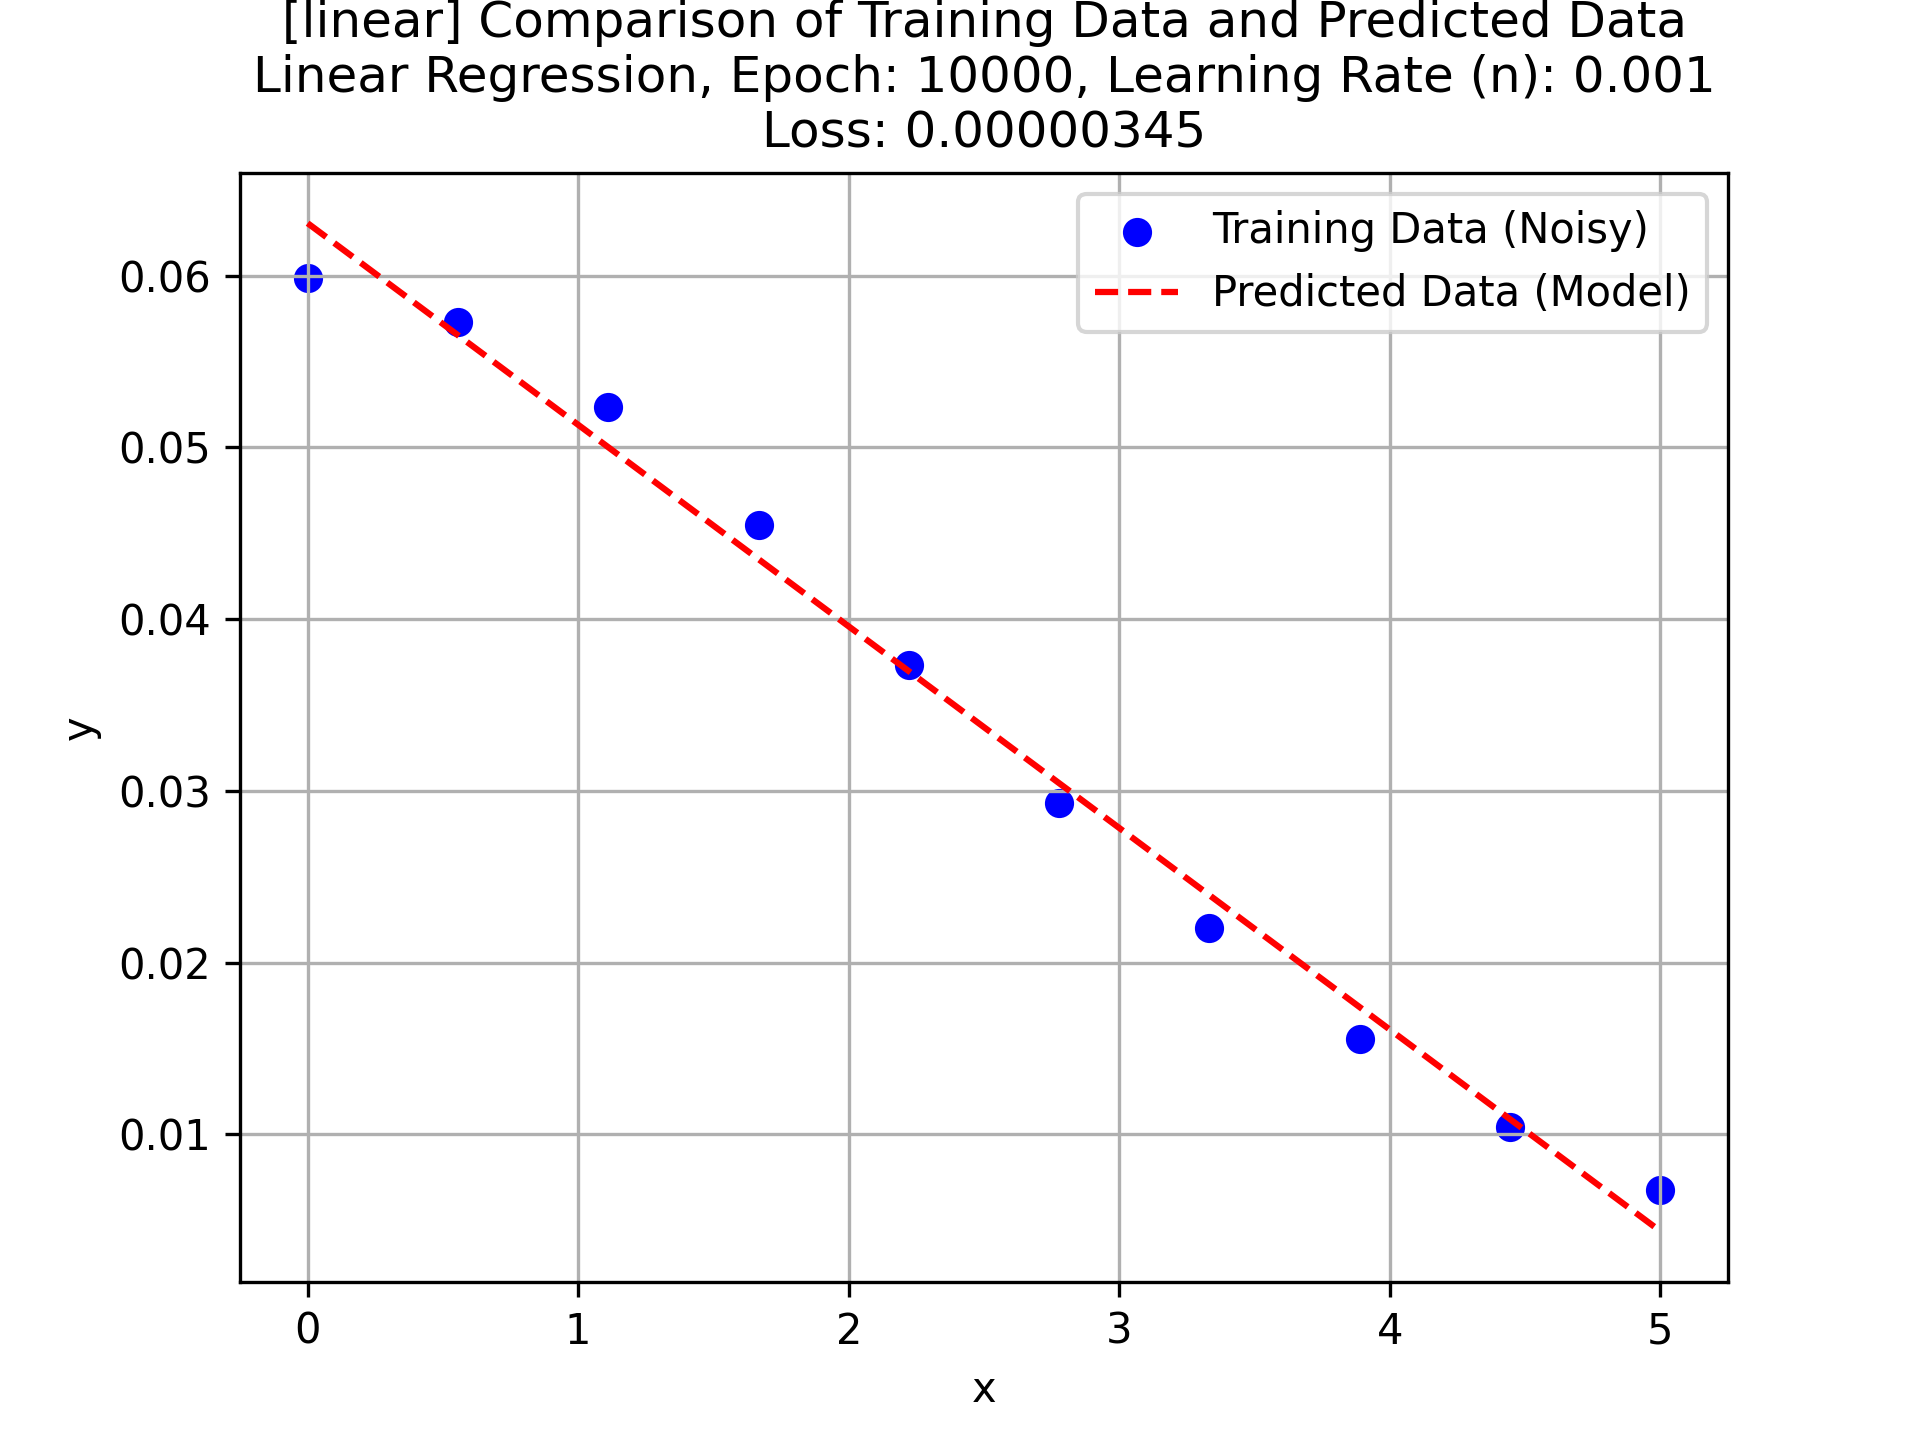
\includegraphics[width=0.8\linewidth]{../Figures/linear_regression_e_10000_n_0.001.png}
   \caption{TPredicted values $y_red$ versus actual data $y$}
   \label{fig:Lin_a}
\end{figure}


\subsection{Problem 1b: Experiment with the learning rate and number of epochs}
Here I tried different values of the learning rate ($\eta$)

%%%%%%%%%%%%%%%%%%%%%%%%%%%%%%%%%%%
\section{Results}

\subsection{General Results}

We observe that the elastic rod begins the simulation as a coiled planar circle, but stretches under gravity to become a helical coil (spring shape).
With the time available for this project, the most accurate simulation of this scenario comprised $N=400$ nodes and $\Delta t = 0.005$ s.
This simulation required 83 mins to complete computation on the author's personal computer.



\subsection{Sensitivity Analysis}

Sensitivity analysis was performed to determine the requirements on the refinement of mesh for accurate results.
The mesh is constructed parametrically by defining the number of nodes $N$ and the time-step in the simulation $\Delta t$.

It is found that decreasing the number of nodes does not have significant impact on the results, as shown in Fig. \ref{fig:lessNodes_zplot}.
However, when we further increase the refinement of $\Delta t: 0.005 \rightarrow 0.001$, there is noticeable difference.
The damping effects on the system in converging to a steady state of $z \approx -0.04$ are less pronounced, and so steady state is not achieved in the $5s$ duration of this simulation.


In either case of adjusting either $K$ or $\Delta t$, the trade off is computational time.
We note that refinement of $\Delta t$ is linearly correlated to the number of steps to be computed. 
In this case, each subsequent step of the simulation should take less iterations of Newton-Raphson to converge as the system approaches a steady state.
Still, as shown in Fig. \ref{fig:lessDT_zplot}, if there is no steady state achieved in the simulation, then the computational time for each step is approximately constant, and so the computational time for this simulation is linearly correlated with the refinement in $\Delta t$.

Alternatively, increasing the density of nodes $K$ has less noticeable effects on computational time, because the physics of nodes that are linked close together mean that there is less variance, and so the computational increase with a higher node density is not a linear correlation; it is intuitively logarithmic in nature.


For completness, we also furnish the nominal plot of z-coordinates in the last node for $N=50$, $\Delta t = 0.01$s, as is furnished in Chapter 7 of the text in this course.

%%%%%%%%%%%%%%%%%%%%%%%%%%%%%%%%%%%
\section*{ACKNOWLEDGMENT}

Material used in this report are taken from the course UCLA MAE 263F, Fall 2024.



%%%%%%%%%%%%%%%%%%%%%%%%%%%%%%%%%%%%%%%%%%%%%%%%%%%%%%%%%%%%%%%%%%%%%%%%%%%%%%%%

\begin{thebibliography}{99}

\bibitem{c1} M. Khalid Jawed, Singmin Lim, Discrete Simulation of Slender Structures, UCLA Fall 2024 MAE 263F

\end{thebibliography}


\end{document}
